\documentclass[master.tex]{subfiles}
\begin{document}

\chapter{Related Work}

There are many proof assistants available out there, each of them rely on
slightly different meta-theory. We can separate proof assistants into 2
categories as the following

\section{Text-Base Proof Assistants}

Text-base proof assistants are similar to programming language where user writes
everything in text-files and compile it, if the compilation is successful, then
the proofs are correct. User can freely manipulate these text-files, hence,
easier to write a complex proof. In addition, most of proof assistants have a
plug-in to mainstream text editor, so user can use their favourite text editor
with full performance.

There are several mainstream text-base proof assistants that worth mentioning

\subsection{Coq}
Coq\supercite{coq-official-website} is one the most famous proof assistants. It
is based on the Calculus of Inductive Constructions (CIC)\footcite{CIC is itself
  is developed alongside Coq.} developed by Thierry
Coquand\supercite{thierry-coquand-homepage}.

Coq has customisable tactics which are commands that transform goal into
smaller-sub goal (if any), this makes proving process become faster compared to
other proof assistants. In contrast, tactics reduce readability, reader might
need to replay each tactic step by step in order to understand a proof
completely.

Coq is very mature, it has been developed since 1984. Hence, it is reliable and
has lots of libraries supported.

In term of editor, most people use Proof
General\supercite{proof-general-official-website} which is a plugin on
Emacs\footnote{Proof General also other proof assistants such as Isabelle and PhoX}.
Nevertheless, Coq has its own editor called
CoqIde\supercite{coqide-official-website} that newcomers can use without
learning Emacs.

\begin{figure}[H]
    \centering
    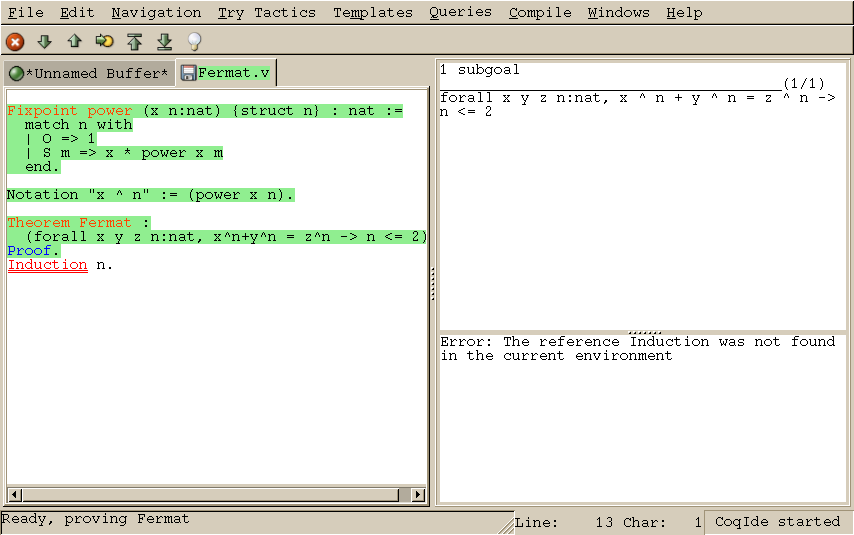
\includegraphics[width=\textwidth]{related-work-coq}
    \caption{Screenshot of Coq (using CoqIde) --- The left pane is file content
      and Upper right pane is the current goal which is changed depending on
      where the cursor point on file content.}
\label{fig:background-coq}
\end{figure}

\subsection{Agda}
Adga\supercite{agda-official-website} is (dependently typed) functional
programming which can be seen as a proof assistant as well. It is based on
Unified Theory of Dependent
Types\supercite{norell:thesis}\supercite{Luo:1994:CRT:184757} similar to Martin
Lof Type Theory.

Its proving technique is relies on Curry-Howard correspondence
which state that there is duality between computer programs and mathematical
proofs\supercite{curry-howard-correspondence}, for example function corresponded
to implication, product type corresponded to logical implication.

Agda is suitable for reasoning about functional programs because we can write a
program and prove that curtain properties of a function hold using the same
language. This is feasible since a proof is just a function due to Curry-Howard
correspondence.

Agda has less steep learning curve compared other proof assistants such as Coq.
This is because user doesn't need to learn about proving
system since it is the same as programming. In contrast, it doesn't have
fancy tactic system so proving process is slower.

In term of popularity, it is less popular than Coq, however, some project such
as Homotopy Type Theory\supercite{hott-coq-repo}\supercite{hott-agda-repo} use
Agda as alternative experiments to Coq.

In term of editor, Agda as its own plugin for Emacs which is very nice but user
need to be familiar to Emacs before using it. There is no alternative plugin to
other editor.

\begin{figure}[H]
    \centering
    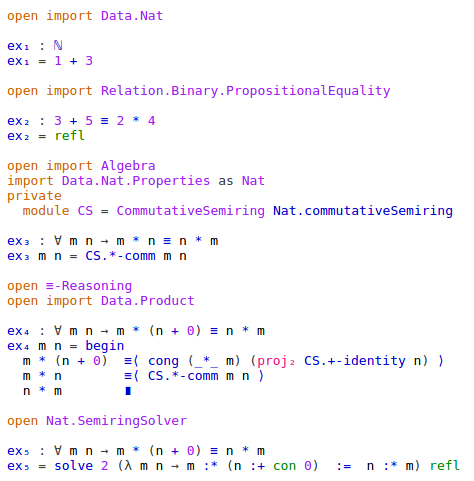
\includegraphics[width=0.6\textwidth]{related-work-agda}
    \caption{Screenshot of Agda --- Credit: an example in Agda standard library,
    removing comment out to save space.}
\label{fig:background-agda}
\end{figure}


\subsection{Isabelle}

Isabelle\supercite{isabelle-official-website} is generic proof assistant.



talk about isabelle readability

\subsection{Lean}
Lean\supercite{lean-offical-website} is a relatively new theorem
prover\footnote{The Lean project was launched by Leonardo de Moura at Microsoft
  Research in 2013} TODO:

\section{Visualised Proof Assistant}
TODO:

\subsection{Logitext}
http://logitext.mit.edu/tutorial
TODO:

\subsection{Panda}
https://www.irit.fr/panda/
TODO:

\subsection{Pandora}
http://www.doc.ic.ac.uk/pandora/newpandora/
TODO:

\subsection{PeaCoq}
http://goto.ucsd.edu/peacoq/
TODO:

\subsection{Why3}
http://why3.lri.fr/
TODO:

\end{document}